\begin{scanpage}{0172}{154}
\begin{center}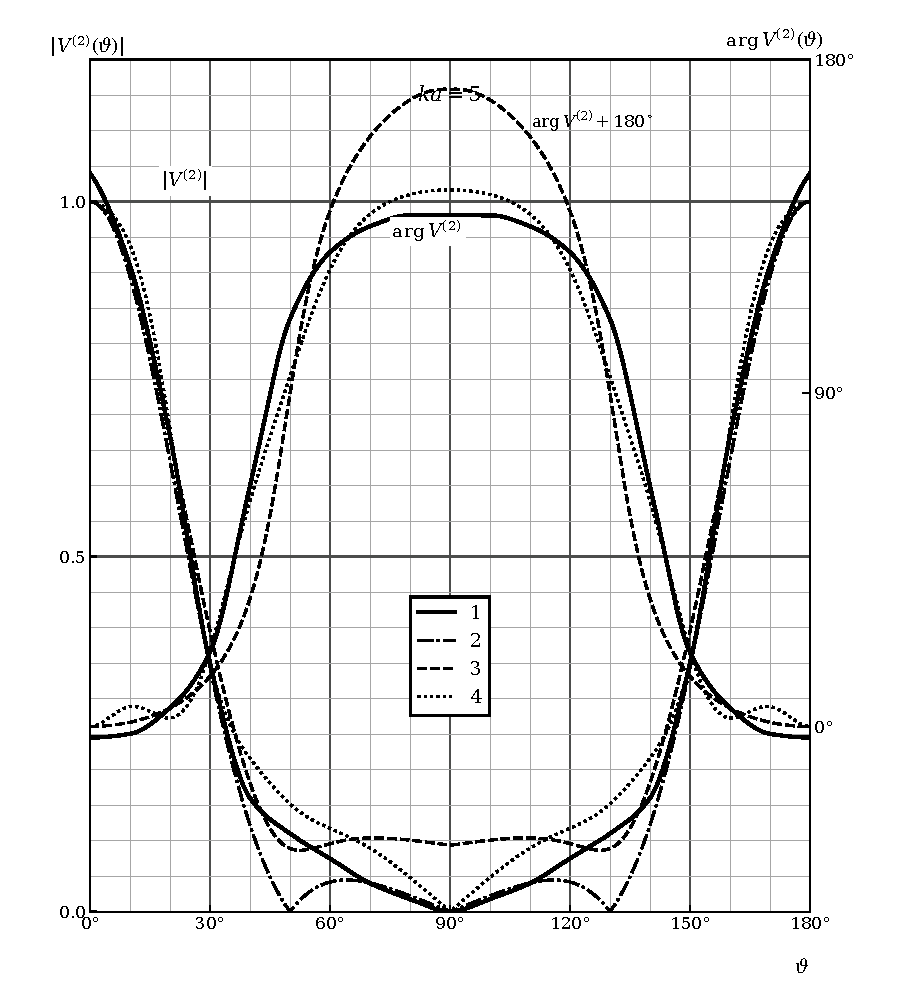
\includegraphics[width=.60\linewidth]{images/recreated/c-0172-fig68.pdf}\par
Figure 68. The function $V^{(2)}(\vartheta)$ for a disk with the normal incidence of a plane wave (curve 4). Curves 1, 2 and 3 from Figure 21 are drawn for comparison
\end{center}
of only secondary waves. In Chapter VII we will investigate the problem of a dipole in which the edge waves decrease so slowly that it is necessary to consider multiple diffraction.
\sectiontitle{25}{A Brief Review of the Literature}
In this and previous chapters, approximation expressions were obtained for the scattering characteristics of a plane wave by various bodies. These expressions were derived with the help of physical considerations which do not pretend to be mathematically rigorous, and they are adequate for sufficiently short waves. In the literature,
\end{scanpage}
